\chapter{Multiple Integrals}

Back in Chapter~20 we built the single integral $\int_a^b f(x)\,\dd x$ out of one
stubbornly simple idea: chop the interval $[a,b]$ into tiny pieces, build a thin
rectangle over each piece, add up their areas, and watch the sum settle onto a
number as the pieces shrink. The picture was a curve over a line, and the answer
was the area trapped between them.

Now the domain grows a dimension. Instead of integrating over an interval on the
$x$-axis, we integrate over a \emph{region} in the $xy$-plane -- a disk, a
triangle, a blob bounded by two curves. The graph of our function $f(x,y)$ is no
longer a curve but a \emph{surface} floating above that region, and the thing we
add up is no longer area but \emph{volume}: the volume of the solid trapped
between the region on the floor and the surface overhead.

Astonishingly, almost nothing new has to be invented. The whole chapter is the
same one idea -- chop, multiply, add, take the limit -- carried into two and
three dimensions. The genuinely new questions are practical ones. How do you
actually \emph{compute} a sum over a two-dimensional region without drowning in
it? (Answer: do it one direction at a time -- that is Fubini's theorem.) And
when the region is round, or the function lives most naturally in some other
coordinate system, how do you change coordinates without corrupting the volume?
(Answer: the Jacobian, which turns out to be a determinant, which turns out to be
exactly the area-scaling factor you met in linear algebra.) Those two ideas --
\textbf{iteration} and \textbf{change of variables} -- are the heart of this
chapter.

\begin{focusbox}
A single integral adds a function over an \emph{interval} and measures
\emph{area}. A double integral adds a function over a \emph{planar region} and
measures \emph{volume}. The definition is the same Riemann sum, just with little
patches of area $\Delta A$ instead of little widths $\Delta x$. Everything hard
is bookkeeping: how to organize the sum (Fubini) and how to bend the coordinate
grid without losing track of area (the Jacobian).
\end{focusbox}

\chapterline

\section{The double integral as volume and as accumulation}
\label{ch34:double}

\subsection{Two readings of the same sum}

When you met $\int_a^b f(x)\,\dd x$ you learned to read it two ways at once, and
both readings will carry over. The \emph{geometric} reading: it is the signed
area under the graph of $f$. The \emph{accumulation} reading: if $f(x)$ is a
density-per-unit-length, then the integral is the total stuff. A double integral
has exactly these same two faces.

\textbf{Geometric reading.} Let $R$ be a region in the $xy$-plane and let
$f(x,y)\ge 0$ be a function defined on it. The graph $z=f(x,y)$ is a surface
hovering above the plane. The double integral
\[
  \iint_R f(x,y)\,\dd A
\]
is the \emph{volume} of the solid that sits over $R$ and reaches up to the
surface. When $f$ dips below zero the contribution is negative, exactly as area
went negative for the single integral when the curve dipped below the axis.

\textbf{Accumulation reading.} Suppose a flat metal plate occupies the region
$R$, and $f(x,y)$ is its \emph{density} -- grams per square centimetre -- which
may vary from point to point. Then $\iint_R f\,\dd A$ is the total \emph{mass} of
the plate. Here there is no surface and no volume in sight; we are simply adding
up a quantity that is spread out over an area, weighting each tiny patch by how
much stuff sits on it. Population over a county, rainfall over a watershed,
charge over a sheet -- all the same integral.

\begin{intuitionbox}
Think of $\dd A$ as an \emph{infinitesimal tile} of the floor, and $f(x,y)$ as
``how tall the building is'' (volume reading) or ``how heavy this tile is''
(mass reading) at that spot. The integral lays down infinitely many infinitely
small tiles over the whole region, multiplies each by its height-or-weight, and
sums. The $\iint$ -- a double S -- is just two nested ``sum'' signs, one for each
direction you have to sweep across the floor.
\end{intuitionbox}

\subsection{The Riemann sum, built honestly}

Let us build the thing from scratch so the definition is not a mystery. To keep
the picture clean, start with a region that is a rectangle,
$R=[a,b]\times[c,d]$ -- all points $(x,y)$ with $a\le x\le b$ and $c\le y\le d$.

Cut $[a,b]$ into $m$ equal sub-intervals of width $\Delta x=(b-a)/m$, and cut
$[c,d]$ into $n$ equal sub-intervals of height $\Delta y=(d-c)/n$. The grid lines
slice $R$ into $m\cdot n$ little rectangles, each of area
\[
  \Delta A=\Delta x\,\Delta y .
\]
In the $(i,j)$-th little rectangle pick any sample point
$(x_i^\ast,\,y_j^\ast)$. Over that rectangle, build a thin rectangular
\emph{box} whose base is the little rectangle and whose height is the value of
the function there, $f(x_i^\ast,y_j^\ast)$. The volume of that one box is
height times base area,
\[
  f(x_i^\ast,y_j^\ast)\,\Delta A .
\]
Now add up all $m\cdot n$ boxes. You get a lumpy, blocky approximation to the
solid under the surface -- a city of skyscrapers approximating a smooth hill:
\[
  S_{m,n}=\sum_{i=1}^{m}\sum_{j=1}^{n} f(x_i^\ast,y_j^\ast)\,\Delta A .
\]
This double sum is the two-dimensional Riemann sum.

\begin{figure}[H]
\centering
\begin{tikzpicture}[scale=1.0]
  \draw[->] (-0.3,0) -- (5,0) node[right] {$x$};
  \draw[->] (0,-0.3) -- (0,3.6) node[above] {$y$};
  \foreach \i in {0,1,2,3,4} {
    \draw[gray!55] (\i,0) -- (\i,3);
  }
  \foreach \j in {0,1,2,3} {
    \draw[gray!55] (0,\j) -- (4,\j);
  }
  \fill[areafill,opacity=0.7] (2,1) rectangle (3,2);
  \node at (2.5,1.5) {\scriptsize $\Delta A$};
  \draw[<->] (0,-0.45) -- (1,-0.45) node[midway,below] {\scriptsize $\Delta x$};
  \draw[<->] (-0.45,0) -- (-0.45,1) node[midway,left] {\scriptsize $\Delta y$};
  \node[below] at (2,-0.05) {\scriptsize $R=[a,b]\times[c,d]$};
\end{tikzpicture}
\caption{The floor $R$ is diced into little tiles of area
$\Delta A=\Delta x\,\Delta y$. Over each tile we erect a box of height
$f(x_i^\ast,y_j^\ast)$. The total box-volume is the Riemann sum
$\sum\sum f\,\Delta A$, which closes in on the true volume as the tiles shrink.}
\label{ch34:fig-grid}
\end{figure}

If, as we make the grid finer and finer ($m,n\to\infty$, so
$\Delta x,\Delta y\to 0$), this sum approaches one and the same number no matter
how we chose the sample points, we call that number the \textbf{double integral}.

\begin{definition}[Double integral over a rectangle]
\label{ch34:def-double}
Let $f$ be defined on $R=[a,b]\times[c,d]$. If the Riemann sums $S_{m,n}$ above
converge to a single limit $L$ as $m,n\to\infty$, independent of the choice of
sample points, then $f$ is \emph{integrable} on $R$ and we write
\[
  \iint_R f(x,y)\,\dd A=L .
\]
\end{definition}

As with one variable, every \emph{continuous} function on a closed bounded region
is integrable -- the proof is the higher-dimensional twin of the one in
Chapter~20 and we will not belabor it. The moral is the same: continuity is
plenty to guarantee the city of skyscrapers settles onto a definite volume.

\begin{happeningbox}
What is $\dd A$ \emph{really}? It is the ghost of $\Delta A=\Delta x\,\Delta y$
after the limit. In the sum you genuinely multiply a width by a height to get a
patch of \emph{area}, and you weight $f$ by that patch. After the limit we write
$\dd A$ to remember ``an infinitesimal patch of area.'' The reason $\dd A$ will
sometimes appear as $\dd x\,\dd y$, sometimes as $r\,\dd r\,\dd\theta$, and
sometimes as something stranger is that those are different honest ways of
measuring the \emph{area of one little patch} depending on how you have sliced
the region. The entire change-of-variables story later in this chapter is one
long answer to the question: ``in these coordinates, how big is one little
patch?''
\end{happeningbox}

\subsection{Regions that are not rectangles}

Real regions are rarely rectangles. To integrate over a triangle or a disk, do
the obvious thing: pretend $f$ is zero outside the region. Enclose the region $R$
inside a big rectangle, define a new function that equals $f$ on $R$ and equals
$0$ everywhere else in the rectangle, and integrate \emph{that} over the
rectangle. Tiles that fall outside $R$ contribute nothing; tiles inside
contribute $f\,\Delta A$ as before. The boundary tiles, the ones the curve slices
through, are a vanishing fraction of the total as the grid shrinks, so they do
not corrupt the limit. This little trick lets Definition~\ref{ch34:def-double}
cover any reasonable region without new ideas.

\begin{focusbox}
Useful sanity checks you will use constantly:
\begin{itemize}
\item $\displaystyle\iint_R 1\,\dd A=\text{area of }R$. (Height $1$ everywhere,
so the ``volume'' is just area times height $=$ area.)
\item $\displaystyle\iint_R c\,f\,\dd A=c\iint_R f\,\dd A$ and the integral of a
sum is the sum of the integrals -- linearity, inherited straight from the sums.
\item If $R$ splits into two non-overlapping pieces $R_1$ and $R_2$, then
$\iint_R=\iint_{R_1}+\iint_{R_2}$. Cut the region, add the volumes.
\end{itemize}
\end{focusbox}

\section{Iterated integrals and Fubini's theorem}
\label{ch34:fubini}

A double sum $\sum_i\sum_j$ is intimidating only until you remember you are
allowed to do the two sums \emph{one at a time}. Fix a column, add up that
column, then add up the column-totals. The continuous version of that simple
regrouping is the single most useful computational fact in this chapter:
\textbf{Fubini's theorem}, which says a double integral can be evaluated as two
ordinary single integrals, nested.

\subsection{The idea: volume by slices}

Here is the picture that makes Fubini obvious. You already know one way to find a
volume from Chapter~26: slice the solid into thin slabs and add the slab volumes.

Take our solid under $z=f(x,y)$ over the rectangle $[a,b]\times[c,d]$. Slice it
with a plane $x=\text{const}$, perpendicular to the $x$-axis. The slice is a thin
slab. Its \emph{cross-sectional area} is the area under the curve
$z=f(x,y)$ as $y$ runs from $c$ to $d$ -- with $x$ held fixed -- which is just a
single integral,
\[
  A(x)=\int_c^d f(x,y)\,\dd y .
\]
The slab has thickness $\dd x$, so its volume is $A(x)\,\dd x$. Add up the slabs
from $x=a$ to $x=b$:
\[
  \text{Volume}=\int_a^b A(x)\,\dd x
             =\int_a^b\!\left(\int_c^d f(x,y)\,\dd y\right)\dd x .
\]
That nested expression is an \emph{iterated integral}. We just sliced the solid
the long way and added the slices.

\begin{figure}[H]
\centering
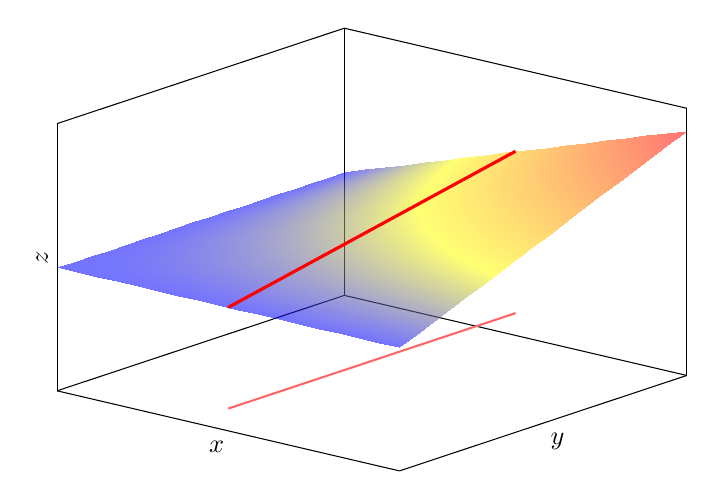
\begin{tikzpicture}[scale=0.95]
  \begin{axis}[
    view={40}{25},
    width=10cm, height=7.5cm,
    xlabel={$x$}, ylabel={$y$}, zlabel={$z$},
    domain=0:2, y domain=0:2,
    samples=18, samples y=18,
    xtick=\empty, ytick=\empty, ztick=\empty,
  ]
    \addplot3[surf, opacity=0.55, shader=interp]
      {2 + 0.6*x*y};
    \addplot3[draw=red, very thick, samples=30, samples y=1, domain=0:2]
      ({1},{x},{2+0.6*1*x});
    \addplot3[draw=red!60, thick, samples=2, samples y=1, domain=0:2]
      ({1},{x},{0});
  \end{axis}
\end{tikzpicture}
\caption{Slicing the solid at a fixed $x$ gives a slab whose face area is
$A(x)=\int_c^d f(x,y)\,\dd y$ (the red profile). Adding the slabs
$A(x)\,\dd x$ from $a$ to $b$ rebuilds the volume. That is Fubini.}
\label{ch34:fig-slice}
\end{figure}

But we could just as well have sliced the \emph{other} way, with planes
$y=\text{const}$, giving
\[
  \text{Volume}=\int_c^d\!\left(\int_a^b f(x,y)\,\dd x\right)\dd y .
\]
The solid does not care which way you slice it. Both iterated integrals equal the
same volume, hence equal each other. That equality -- and the fact that either
equals the genuine double integral $\iint_R f\,\dd A$ -- is the content of
Fubini.

\begin{theorem}[Fubini, for nice functions]
\label{ch34:thm-fubini}
If $f$ is continuous on the rectangle $R=[a,b]\times[c,d]$, then
\[
  \iint_R f(x,y)\,\dd A
  =\int_a^b\!\int_c^d f(x,y)\,\dd y\,\dd x
  =\int_c^d\!\int_a^b f(x,y)\,\dd x\,\dd y .
\]
In particular both orders of integration give the same answer, and both equal the
double integral.
\end{theorem}

\begin{whybox}
Why is the iterated integral allowed to replace the double sum at all? Because
addition does not care how you group it. In the Riemann sum
$\sum_i\sum_j f(x_i^\ast,y_j^\ast)\,\Delta x\,\Delta y$, factor the constant
$\Delta x$ out of the inner sum:
\[
  \sum_i\Big(\underbrace{\sum_j f(x_i^\ast,y_j^\ast)\,\Delta y}_{\approx\,A(x_i^\ast)}\Big)\Delta x .
\]
The inner sum is a Riemann sum in $y$ alone; as the grid refines it becomes
$\int_c^d f(x_i^\ast,y)\,\dd y=A(x_i^\ast)$. The outer sum is then a Riemann sum
of $A(x)$ in $x$, becoming $\int_a^b A(x)\,\dd x$. So Fubini is nothing but
``do the $y$-sum first, then the $x$-sum,'' the freedom to regroup a sum, carried
through the limit. The one piece of fine print -- which is why Fubini is a
\emph{theorem} and not a triviality -- is checking that the limits can be taken
in this nested order; continuity (more generally, $\iint|f|\,\dd A<\infty$) is
what licenses it.
\end{whybox}

\begin{historybox}
The theorem is named for Guido Fubini, who proved a sweeping version in 1907
within Lebesgue's new theory of integration. But the practice is far older:
Newton, the Bernoullis, and Euler computed volumes by iterated integration as a
matter of course in the 1600s and 1700s, slicing solids and adding the slices
without a worry. What the twentieth century added was the precise hypothesis --
that $f$ be absolutely integrable -- under which the cavalier swapping of
integration order is \emph{guaranteed} safe. It is not always safe: there are
functions (non-integrable in absolute value) for which the two orders give
genuinely different answers. Continuity on a bounded region spares you all such
pathology, which is why every example in this book swaps freely.
\end{historybox}

\subsection{A first computation}

\begin{example}[A double integral over a rectangle]
\label{ch34:ex-rect}
Compute $\displaystyle\iint_R (x+2y)\,\dd A$ over $R=[0,2]\times[0,3]$.

Integrate in $y$ first, treating $x$ as a constant:
\[
  \int_0^3 (x+2y)\,\dd y
  =\eval{xy+y^2}{0}^{3}
  =3x+9 .
\]
Now integrate that in $x$:
\[
  \int_0^2 (3x+9)\,\dd x
  =\eval{\tfrac{3}{2}x^2+9x}{0}^{2}
  =6+18=24 .
\]
As a check, slice the other way -- $x$ first:
\[
  \int_0^2 (x+2y)\,\dd x=\eval{\tfrac12 x^2+2xy}{0}^{2}=2+4y,
  \qquad
  \int_0^3 (2+4y)\,\dd y=\eval{2y+2y^2}{0}^{3}=6+18=24 .
\]
Same number, as Fubini promised.
\end{example}

\begin{trapbox}
The bounds and the differentials must match up \emph{from the inside out}. In
$\int_a^b\!\int_c^d f\,\dd y\,\dd x$, the inner differential $\dd y$ pairs with
the inner limits $c,d$, and the outer $\dd x$ pairs with $a,b$. A frequent
disaster is writing the limits in the wrong order, so that $x$ ends up
``integrated'' over $y$'s interval. Read the integral inside-out, like nested
parentheses, and keep each variable with its own bounds.
\end{trapbox}

\subsection{Non-rectangular regions: variable bounds}

For a rectangle the inner limits are constants. For a curvy region they are
\emph{functions}, because the cross-section changes length as you sweep across.
There are two standard shapes.

A region is \emph{$y$-simple} (vertically simple) if it sits between two curves
$y=g_1(x)$ below and $y=g_2(x)$ above, for $x$ in some interval $[a,b]$. Slice it
vertically: at each fixed $x$, $y$ runs from the bottom curve to the top curve.
\[
  \iint_R f\,\dd A=\int_a^b\!\int_{g_1(x)}^{g_2(x)} f(x,y)\,\dd y\,\dd x .
\]
A region is \emph{$x$-simple} (horizontally simple) if it lies between
$x=h_1(y)$ on the left and $x=h_2(y)$ on the right, for $y$ in $[c,d]$:
\[
  \iint_R f\,\dd A=\int_c^d\!\int_{h_1(y)}^{h_2(y)} f(x,y)\,\dd x\,\dd y .
\]

\begin{figure}[H]
\centering
\begin{tikzpicture}[scale=1.5]
  \draw[->] (-0.2,0) -- (2.3,0) node[right] {$x$};
  \draw[->] (0,-0.2) -- (0,2.3) node[above] {$y$};
  \draw[domain=0:1, smooth, variable=\x, curveblue, very thick]
    plot ({2*\x},{2*\x*\x});
  \draw[domain=0:1, smooth, variable=\x, targetgreen, very thick]
    plot ({2*\x},{2*\x});
  \fill[areafill,opacity=0.35]
    plot[domain=0:1,smooth,variable=\x] ({2*\x},{2*\x})
    -- plot[domain=1:0,smooth,variable=\x] ({2*\x},{2*\x*\x})
    -- cycle;
  \draw[red, thick, ->] (1.2,0.72) -- (1.2,1.2);
  \node[red, right] at (1.2,0.95) {\scriptsize slice};
  \node[targetgreen, left] at (1.6,1.75) {\scriptsize $y=g_2(x)$};
  \node[curveblue, right] at (1.55,1.0) {\scriptsize $y=g_1(x)$};
  \node[below] at (0,0) {\scriptsize $a$};
  \draw[gray] (2,0.02) -- (2,-0.02) node[below] {\scriptsize $b$};
\end{tikzpicture}
\caption{A $y$-simple region. A vertical slice at fixed $x$ runs from the lower
curve $y=g_1(x)$ to the upper curve $y=g_2(x)$, so the inner $y$-integral has
those curves as its limits.}
\label{ch34:fig-ysimple}
\end{figure}

\begin{example}[A triangular region]
\label{ch34:ex-tri}
Integrate $f(x,y)=x$ over the triangle $R$ with vertices $(0,0)$, $(1,0)$,
$(1,1)$. The hypotenuse is the line $y=x$; the bottom is $y=0$; the right edge is
$x=1$. Treating $R$ as $y$-simple: for each $x\in[0,1]$, $y$ runs from $0$ up to
$x$.
\[
  \iint_R x\,\dd A=\int_0^1\!\int_0^x x\,\dd y\,\dd x
  =\int_0^1 x\cdot\eval{y}{0}^{x}\,\dd x
  =\int_0^1 x\cdot x\,\dd x
  =\int_0^1 x^2\,\dd x=\frac13 .
\]
\end{example}

\subsection{Changing the order of integration}

Here is where iterated integrals earn their keep. Sometimes one order is
miserable and the reverse order is easy -- or the inner integral in one order has
no elementary antiderivative at all, but flips into something trivial the other
way. The technique is always the same: \textbf{draw the region}, read off the
\emph{other} kind of bounds, and rewrite.

\begin{example}[An integral you cannot do in the given order]
\label{ch34:ex-order}
Evaluate
\[
  I=\int_0^1\!\int_x^1 e^{y^2}\,\dd y\,\dd x .
\]
The inner integral $\int e^{y^2}\,\dd y$ has \emph{no} elementary
antiderivative -- you are stuck cold. So change the order.

First decode the region from the bounds as written: $x$ goes from $0$ to $1$,
and for each $x$, $y$ goes from $y=x$ up to $y=1$. That is the triangle bounded
by $y=x$, $y=1$, and $x=0$ -- the triangle with vertices $(0,0)$, $(0,1)$,
$(1,1)$.

Now describe the \emph{same} triangle as $x$-simple. Let $y$ run from $0$ to $1$;
for each $y$, $x$ runs from the left edge $x=0$ to the right edge $x=y$ (the line
$y=x$ solved for $x$). So
\[
  I=\int_0^1\!\int_0^y e^{y^2}\,\dd x\,\dd y .
\]
Now the inner integral is trivial -- $e^{y^2}$ is constant in $x$:
\[
  \int_0^y e^{y^2}\,\dd x=y\,e^{y^2},
  \qquad
  I=\int_0^1 y\,e^{y^2}\,\dd y .
\]
And \emph{that} we can do, with the substitution $u=y^2$, $\dd u=2y\,\dd y$:
\[
  I=\frac12\int_0^1 e^{u}\,\dd u=\frac12(e-1).
\]
The same region, swept the other direction, turned an impossible integral into a
one-line substitution.
\end{example}

\begin{walkbox}
Take Example~\ref{ch34:ex-order} on your walk. The number $\tfrac12(e-1)$ never
needed the antiderivative of $e^{y^2}$ -- yet the inner integral as first written
\emph{was} that forbidden antiderivative. How can a quantity be perfectly
computable while one route to it is blocked? (Hint: the blocked route asks for
the antiderivative as a \emph{function of $x$}; the open route only ever needs a
\emph{definite} integral, a single number. The double integral is a number; only
our bookkeeping made it look like it needed a forbidden function.)
\end{walkbox}

\begin{trapbox}
When you flip the order, you must re-derive the limits from the \emph{geometry},
not by mechanically swapping the symbols. Swapping
$\int_0^1\!\int_x^1\,\dd y\,\dd x$ into $\int_0^1\!\int_x^1\,\dd x\,\dd y$ is
nonsense -- you cannot have $x$ in the limits of an $x$-integral. Sketch the
region every single time; let the picture tell you the new bounds.
\end{trapbox}

\section{Polar coordinates and the Gaussian integral}
\label{ch34:polar}

Some regions hate the rectangular grid. A disk, an annulus, a circular sector --
their natural description is ``radius from here to there, angle from here to
there,'' not ``$x$ from here to there.'' For these, switch to \textbf{polar
coordinates}
\[
  x=r\cos\theta,\qquad y=r\sin\theta,
\]
where $r\ge 0$ is the distance from the origin and $\theta$ is the angle. A disk
of radius $a$ is simply $0\le r\le a$, $0\le\theta\le 2\pi$ -- a rectangle in the
$(r,\theta)$ world.

\subsection{The crucial factor of $r$}

Here is the subtlety that trips up everyone the first time. In rectangular
coordinates, $\dd A=\dd x\,\dd y$, because a little grid cell is a tiny rectangle
of width $\dd x$ and height $\dd y$. In polar coordinates, $\dd A$ is
\[
  \boxed{\;\dd A=r\,\dd r\,\dd\theta\;}
\]
\emph{not} $\dd r\,\dd\theta$. There is an extra factor of $r$, and the whole
chapter's payoff is understanding where it comes from -- because it is the first
appearance of the change-of-variables idea that will close the chapter.

\begin{happeningbox}
Picture the polar grid: circles of constant $r$ and rays of constant $\theta$.
The little cell between radius $r$ and $r+\dd r$, and between angle $\theta$ and
$\theta+\dd\theta$, is \emph{not} a rectangle of sides $\dd r$ and $\dd\theta$.
Its two ``radial'' sides do have length $\dd r$. But its two ``arc'' sides are
pieces of circles, and the length of a circular arc is radius times angle:
$r\,\dd\theta$. So the cell is (very nearly) a rectangle of sides $\dd r$ and
$r\,\dd\theta$, with area
\[
  \dd A=(\dd r)(r\,\dd\theta)=r\,\dd r\,\dd\theta .
\]
The factor $r$ is the confession that polar cells \emph{grow} as you move
outward: a cell spanning one degree of angle is tiny near the origin and huge far
away, in exact proportion to $r$. Forgetting the $r$ is the single most common
error in polar integration, and now you know it is not a rule to memorize but an
arc length to remember.
\end{happeningbox}

\begin{figure}[H]
\centering
\begin{tikzpicture}[scale=1.0]
  \foreach \a in {15,30,45,60,75} {
    \draw[gray!55] (0,0) -- (\a:3.3);
  }
  \foreach \r in {1,1.7,2.4,3.1} {
    \draw[gray!55] (12:\r) arc (12:78:\r);
  }
  \fill[areafill,opacity=0.6] (30:1.7) -- (30:2.4)
     arc (30:45:2.4) -- (45:1.7) arc (45:30:1.7) -- cycle;
  \draw[red,thick] (30:1.7) -- (30:2.4);
  \node[red,right] at (29:2.05) {\scriptsize $\dd r$};
  \draw[blue,thick] (30:2.4) arc (30:45:2.4);
  \node[blue,right] at (37:2.55) {\scriptsize $r\,\dd\theta$};
  \draw[->] (0,0) -- (0:3.5) node[right] {$x$};
  \node at (8:0.55) {\scriptsize $\theta$};
\end{tikzpicture}
\caption{A polar grid cell is bounded by two rays and two arcs. Its radial side
has length $\dd r$; its arc side has length $r\,\dd\theta$. Hence
$\dd A=r\,\dd r\,\dd\theta$. The cells fan out -- bigger at larger $r$ -- and the
factor $r$ records exactly that.}
\label{ch34:fig-polar}
\end{figure}

So the conversion rule is: replace $x\to r\cos\theta$, $y\to r\sin\theta$, and
$\dd x\,\dd y\to r\,\dd r\,\dd\theta$, then set the limits as $r$- and
$\theta$-ranges.
\[
  \iint_R f(x,y)\,\dd x\,\dd y
  =\iint_{R'} f(r\cos\theta,\,r\sin\theta)\;r\,\dd r\,\dd\theta .
\]

\begin{example}[Area of a disk, the honest way]
\label{ch34:ex-disk}
Take $f=1$ over the disk of radius $a$. In polar:
\[
  \iint_R 1\,\dd A=\int_0^{2\pi}\!\int_0^a 1\cdot r\,\dd r\,\dd\theta
  =\int_0^{2\pi}\eval{\tfrac12 r^2}{0}^{a}\,\dd\theta
  =\int_0^{2\pi}\frac{a^2}{2}\,\dd\theta=\pi a^2 .
\]
There is $\pi a^2$, falling straight out -- and notice the $r$ was essential.
Without it you would have integrated $\int_0^a \dd r=a$ and gotten the
nonsensical $2\pi a$.
\end{example}

\subsection{The Gaussian integral: a small miracle}

We can now compute one of the most important integrals in all of mathematics --
the one underneath the bell curve, statistics, the heat equation, and quantum
mechanics:
\[
  I=\int_{-\infty}^{\infty} e^{-x^2}\,\dd x .
\]
The function $e^{-x^2}$ has \emph{no} elementary antiderivative (we noted its
cousin $e^{y^2}$ in Example~\ref{ch34:ex-order}). The one-variable methods of
this book cannot touch it. Yet the answer is exactly $\sqrt{\pi}$, and the trick
that gets it -- due in spirit to Poisson and Laplace -- is a jewel: \emph{square
the integral and read it as a double integral, then go polar.}

\begin{example}[$\int_{-\infty}^\infty e^{-x^2}\,\dd x=\sqrt\pi$]
\label{ch34:ex-gauss}
We cannot find $I$ directly, so consider $I^2$. Because the integral is just a
number, we may name the dummy variable of the second copy differently -- call it
$y$:
\[
  I^2=\left(\int_{-\infty}^\infty e^{-x^2}\,\dd x\right)
      \left(\int_{-\infty}^\infty e^{-y^2}\,\dd y\right)
     =\int_{-\infty}^\infty\!\int_{-\infty}^\infty e^{-x^2}e^{-y^2}\,\dd x\,\dd y .
\]
The step that does the magic: $e^{-x^2}e^{-y^2}=e^{-(x^2+y^2)}$. The integrand
depends on $x$ and $y$ only through $x^2+y^2=r^2$ -- it is \emph{radially
symmetric}. That is the flashing sign that polar coordinates will collapse it.
The region is the whole plane, so $r$ runs $0$ to $\infty$ and $\theta$ runs $0$
to $2\pi$. With $x^2+y^2=r^2$ and the mandatory $\dd A=r\,\dd r\,\dd\theta$:
\[
  I^2=\int_0^{2\pi}\!\int_0^\infty e^{-r^2}\,r\,\dd r\,\dd\theta .
\]
Now the factor of $r$ -- which we were forced to include -- is exactly the factor
that makes the radial integral elementary. Substitute $u=r^2$, $\dd u=2r\,\dd r$:
\[
  \int_0^\infty e^{-r^2}\,r\,\dd r
  =\frac12\int_0^\infty e^{-u}\,\dd u
  =\frac12\,\eval{-e^{-u}}{0}^{\infty}=\frac12 .
\]
Therefore
\[
  I^2=\int_0^{2\pi}\frac12\,\dd\theta=\frac12\cdot 2\pi=\pi,
  \qquad\Longrightarrow\qquad
  I=\sqrt\pi .
\]
\end{example}

\begin{aestheticbox}
Savor what just happened. A one-dimensional integral that \emph{provably} has no
elementary antiderivative was conquered by stepping \emph{up} into two
dimensions, where its radial symmetry could be seen, and the unavoidable polar
factor $r$ -- the very thing students forget -- was precisely the missing piece
that an antiderivative needs. The problem was unsolvable not because it was
hard but because it was viewed in too few dimensions. Going up a dimension to
solve a lower-dimensional problem is one of the great recurring moves in
mathematics, and here you have watched it produce $\sqrt\pi$ out of thin air.
\end{aestheticbox}

\begin{applicationbox}
The bell curve of statistics is $\frac{1}{\sqrt{2\pi}\,\sigma}
e^{-(x-\mu)^2/2\sigma^2}$. The strange-looking constant $\frac{1}{\sqrt{2\pi}}$
is there for exactly one reason: so the total probability integrates to $1$.
Substituting and using $I=\sqrt\pi$ is what forces that normalizing constant.
Every time a statistician, physicist, or machine-learning engineer writes down a
Gaussian, the $\sqrt{2\pi}$ they carry around is a direct descendant of the polar
computation you just did.
\end{applicationbox}

\section{Triple integrals}
\label{ch34:triple}

Add one more dimension and nothing conceptually changes. A \textbf{triple
integral}
\[
  \iiint_E f(x,y,z)\,\dd V
\]
chops a solid region $E\subset\R^3$ into tiny boxes of volume
$\dd V=\dd x\,\dd y\,\dd z$, weights each by $f$, and sums. Fubini still holds:
evaluate it as three nested single integrals, in any of the six orders, with the
inner limits possibly functions of the outer variables.

\subsection{What it measures}

If $f=1$, the triple integral is the \emph{volume} of $E$:
$\iiint_E 1\,\dd V=\text{Vol}(E)$. (Just as $\iint 1\,\dd A$ was area.) If $f$ is
a density -- mass per unit volume -- the integral is the total \emph{mass} of a
solid body. There is no ``graph'' picture this time, because the graph
$w=f(x,y,z)$ would live in four dimensions; the accumulation reading is the one
to hold onto. We are summing a quantity spread through a three-dimensional body.

\begin{example}[Volume of a tetrahedron]
\label{ch34:ex-tet}
Find the volume of the solid $E$ bounded by the coordinate planes and the plane
$x+y+z=1$ (the corner of the unit cube cut by a slanted plane). Sweep $z$ first:
for fixed $(x,y)$ in the base triangle, $z$ runs from the floor $z=0$ up to the
slanted roof $z=1-x-y$. The base triangle (where the roof is still above the
floor, i.e.\ $1-x-y\ge 0$) is $0\le y\le 1-x$, $0\le x\le 1$. So
\[
  \text{Vol}(E)=\int_0^1\!\int_0^{1-x}\!\int_0^{1-x-y} 1\,\dd z\,\dd y\,\dd x .
\]
Innermost: $\int_0^{1-x-y}\dd z=1-x-y$. Middle:
\[
  \int_0^{1-x}(1-x-y)\,\dd y
  =\eval{(1-x)y-\tfrac12 y^2}{0}^{1-x}
  =(1-x)^2-\tfrac12(1-x)^2=\tfrac12(1-x)^2 .
\]
Outermost, with $u=1-x$:
\[
  \int_0^1\tfrac12(1-x)^2\,\dd x=\frac12\int_0^1 u^2\,\dd u=\frac12\cdot\frac13=\frac16 .
\]
The volume is $\tfrac16$, the familiar volume of that corner tetrahedron.
\end{example}

\begin{labbox}
Confirm $\tfrac16$ a second way. Treat the tetrahedron as a stack of horizontal
triangular slices at height $z$. At height $z$, the cross-section is the triangle
$x+y\le 1-z$, $x,y\ge 0$, a right triangle of legs $1-z$, so of area
$\tfrac12(1-z)^2$. Then $\text{Vol}=\int_0^1\tfrac12(1-z)^2\,\dd z=\tfrac16$.
Two slicing orders, one answer -- Fubini in three dimensions, by hand.
\end{labbox}

\subsection{Cylindrical and spherical coordinates}

Just as planar disks begged for polar coordinates, round solids beg for
\emph{cylindrical} or \emph{spherical} coordinates, and the same ``how big is one
little cell?'' question fixes the volume element.

\textbf{Cylindrical} coordinates are just polar in the $xy$-plane with $z$ left
alone: $x=r\cos\theta$, $y=r\sin\theta$, $z=z$. A cell is a polar cell
($r\,\dd r\,\dd\theta$ of floor area) times a height $\dd z$, so
\[
  \dd V=r\,\dd r\,\dd\theta\,\dd z .
\]
The same factor $r$ as before, for the same arc-length reason.

\textbf{Spherical} coordinates measure a point by its distance $\rho$ from the
origin, the angle $\phi$ down from the positive $z$-axis (the ``polar angle''),
and the angle $\theta$ around the $z$-axis (the ``azimuth''):
\[
  x=\rho\sin\phi\cos\theta,\quad
  y=\rho\sin\phi\sin\theta,\quad
  z=\rho\cos\phi .
\]
A spherical cell has three edges: a radial edge of length $\dd\rho$; an edge
along the $\phi$ direction, which is an arc of a circle of radius $\rho$, of
length $\rho\,\dd\phi$; and an edge along the $\theta$ direction, which is an arc
of a circle of radius $\rho\sin\phi$ (the distance from the $z$-axis), of length
$\rho\sin\phi\,\dd\theta$. Multiply the three edge lengths:
\[
  \boxed{\;\dd V=\rho^2\sin\phi\,\dd\rho\,\dd\phi\,\dd\theta\;}
\]

\begin{happeningbox}
Do not memorize $\rho^2\sin\phi$ -- \emph{rebuild} it. The cell is nearly a
little box with three perpendicular edges of lengths $\dd\rho$, $\rho\,\dd\phi$,
and $\rho\sin\phi\,\dd\theta$. Multiplying: $\rho\cdot\rho\sin\phi=\rho^2\sin\phi$
out front, then $\dd\rho\,\dd\phi\,\dd\theta$. Each factor is just an arc length,
``radius times angle,'' for the circle that that coordinate sweeps along. The
$\sin\phi$ appears because circles of constant latitude shrink toward the poles:
near the north pole ($\phi\approx 0$) a full lap in $\theta$ covers almost no
distance, and $\sin\phi\to 0$ records it.
\end{happeningbox}

\begin{example}[Volume of a ball, finally]
\label{ch34:ex-ball}
The ball of radius $a$ is $0\le\rho\le a$, $0\le\phi\le\pi$, $0\le\theta\le 2\pi$
-- a box in spherical coordinates. With $f=1$:
\[
  \text{Vol}=\int_0^{2\pi}\!\int_0^{\pi}\!\int_0^a
     \rho^2\sin\phi\,\dd\rho\,\dd\phi\,\dd\theta .
\]
The three integrals separate because each factor depends on a single variable:
\[
  \int_0^a\rho^2\,\dd\rho=\frac{a^3}{3},\qquad
  \int_0^\pi\sin\phi\,\dd\phi=\eval{-\cos\phi}{0}^{\pi}=2,\qquad
  \int_0^{2\pi}\dd\theta=2\pi .
\]
Multiply: $\text{Vol}=\dfrac{a^3}{3}\cdot 2\cdot 2\pi=\dfrac{4}{3}\pi a^3$. The
famous formula, derived rather than recited.
\end{example}

\section{The Jacobian: change of variables as area scaling}
\label{ch34:jacobian}

We have now twice pulled a mysterious factor out of a hat: $r$ for polar,
$\rho^2\sin\phi$ for spherical. Each time the justification was a hand-drawn
picture of ``how big is one cell.'' It is time to see the \emph{general} law
behind these factors, and to recognize it as an old friend from linear algebra:
the \textbf{determinant}.

\subsection{The one-variable rehearsal}

You already know the seed of this in one dimension; it is just $u$-substitution.
When you substitute $x=g(u)$ in $\int f(x)\,\dd x$, you replace
$\dd x$ by $g'(u)\,\dd u$:
\[
  \int_a^b f(x)\,\dd x=\int_{u_a}^{u_b} f(g(u))\,g'(u)\,\dd u .
\]
The factor $g'(u)$ is a \emph{stretch factor}: near $u$, the map $g$ stretches a
little interval $\dd u$ into an interval of length $|g'(u)|\,\dd u$. (We carry an
absolute value when we ignore orientation and only care about length.) The
substitution rule \emph{is} the statement ``account for how much the
transformation stretches length.''

\begin{whybox}
The Jacobian is this same idea promoted to two and three dimensions. In one
dimension a smooth map stretches lengths by $|g'(u)|$. In two dimensions a smooth
map $(u,v)\mapsto(x,y)$ stretches \emph{areas}, and the local stretch factor is
\emph{not} a single derivative but a determinant of partial derivatives, because
near a point a smooth map looks like a \emph{linear} map, and the factor by which
a linear map scales area is exactly the absolute value of its determinant -- a
fact you proved in linear algebra. Change of variables in a multiple integral is
$u$-substitution with the word ``derivative'' replaced by the word
``determinant,'' for the simple reason that area-scaling in many dimensions is
measured by a determinant.
\end{whybox}

\subsection{Why a determinant: linearization}

Let a transformation $T$ carry the $uv$-plane to the $xy$-plane:
\[
  x=x(u,v),\qquad y=y(u,v).
\]
Take a tiny rectangle in the $uv$-plane with corner at $(u,v)$ and sides
$\dd u$ (along the $u$-axis) and $\dd v$ (along the $v$-axis). Where does $T$ send
it? Each corner moves, and because the rectangle is tiny, $T$ acts on it almost
\emph{linearly}: the image is (very nearly) a parallelogram. The side that was
$\dd u\,\vec{e}_u$ becomes the vector
\[
  \vec{a}=\left(\pdv{x}{u},\,\pdv{y}{u}\right)\dd u,
\]
because moving by $\dd u$ in the $u$-direction changes $x$ by $\pdv{x}{u}\dd u$
and $y$ by $\pdv{y}{u}\dd u$. Likewise the $\dd v$ side becomes
\[
  \vec{b}=\left(\pdv{x}{v},\,\pdv{y}{v}\right)\dd v .
\]
The image cell is the parallelogram spanned by $\vec a$ and $\vec b$, and the area
of a parallelogram spanned by two vectors is the absolute value of the
$2\times 2$ determinant of their components:
\[
  \dd A_{xy}
  =\left|\det\!\begin{pmatrix}\pdv{x}{u} & \pdv{x}{v}\\[4pt]
                              \pdv{y}{u} & \pdv{y}{v}\end{pmatrix}\right|
  \,\dd u\,\dd v .
\]

\begin{figure}[H]
\centering
\begin{tikzpicture}[scale=1.0]
  \begin{scope}
    \draw[->] (-0.2,0)--(2.4,0) node[right]{\scriptsize $u$};
    \draw[->] (0,-0.2)--(0,2.4) node[above]{\scriptsize $v$};
    \fill[areafill,opacity=0.5] (0.7,0.7) rectangle (1.5,1.5);
    \draw (0.7,0.7) rectangle (1.5,1.5);
    \node at (1.1,1.1) {\scriptsize $\dd u\,\dd v$};
  \end{scope}
  \draw[->, very thick, structurepurple] (2.7,1.1) -- (3.9,1.1)
     node[midway,above]{\scriptsize $T$};
  \begin{scope}[xshift=4.4cm]
    \draw[->] (-0.2,0)--(2.6,0) node[right]{\scriptsize $x$};
    \draw[->] (0,-0.2)--(0,2.4) node[above]{\scriptsize $y$};
    \fill[areafill,opacity=0.5] (0.6,0.6) -- (1.7,0.9) -- (2.0,1.8) -- (0.9,1.5) -- cycle;
    \draw (0.6,0.6) -- (1.7,0.9) -- (2.0,1.8) -- (0.9,1.5) -- cycle;
    \draw[->,red,thick] (0.6,0.6)--(1.7,0.9) node[midway,below]{\scriptsize $\vec a$};
    \draw[->,blue,thick] (0.6,0.6)--(0.9,1.5) node[midway,left]{\scriptsize $\vec b$};
  \end{scope}
\end{tikzpicture}
\caption{Under a smooth map $T$, a tiny rectangle becomes a tiny parallelogram.
Its area is $|\det|\;\dd u\,\dd v$, where the determinant is built from the
partial derivatives. That determinant is the Jacobian.}
\label{ch34:fig-jacobian}
\end{figure}

That determinant has a name.

\begin{definition}[Jacobian]
\label{ch34:def-jacobian}
For a transformation $x=x(u,v)$, $y=y(u,v)$, the \emph{Jacobian determinant} is
\[
  \frac{\partial(x,y)}{\partial(u,v)}
  =\det\!\begin{pmatrix}\pdv{x}{u} & \pdv{x}{v}\\[4pt]
                        \pdv{y}{u} & \pdv{y}{v}\end{pmatrix}
  =\pdv{x}{u}\pdv{y}{v}-\pdv{x}{v}\pdv{y}{u}.
\]
\end{definition}

\begin{theorem}[Change of variables]
\label{ch34:thm-cov}
If $T:(u,v)\mapsto(x,y)$ is a smooth, invertible map carrying a region $S$ in the
$uv$-plane onto a region $R$ in the $xy$-plane, then
\[
  \iint_R f(x,y)\,\dd x\,\dd y
  =\iint_S f\big(x(u,v),y(u,v)\big)\,
     \left|\frac{\partial(x,y)}{\partial(u,v)}\right|\dd u\,\dd v .
\]
\end{theorem}

So changing variables in a double integral is: substitute the new expressions for
$x$ and $y$ into $f$, replace $\dd x\,\dd y$ by the absolute Jacobian times
$\dd u\,\dd v$, and re-state the limits in the new variables. It is
$u$-substitution wearing a determinant.

\begin{connectionbox}
This is the moment two big stories in your education shake hands. In linear
algebra you learned that the determinant of a matrix is the factor by which the
corresponding linear map scales area (in 2D) or volume (in 3D), and that a
negative determinant means the map also flips orientation. In calculus you
learned that a smooth map, viewed closely enough, \emph{is} linear -- its
derivative. Put them together: the local area-scaling of a smooth map is the
determinant of its derivative matrix. The Jacobian is the determinant of the
derivative. Two subjects, one idea.
\end{connectionbox}

\subsection{Polar coordinates, re-derived without pictures}

Let us check the machine against an answer we already trust. For polar
coordinates the ``new variables'' are $(r,\theta)$ and
$x=r\cos\theta$, $y=r\sin\theta$. The partials:
\[
  \pdv{x}{r}=\cos\theta,\quad \pdv{x}{\theta}=-r\sin\theta,\quad
  \pdv{y}{r}=\sin\theta,\quad \pdv{y}{\theta}=r\cos\theta .
\]
The Jacobian:
\[
  \frac{\partial(x,y)}{\partial(r,\theta)}
  =\det\!\begin{pmatrix}\cos\theta & -r\sin\theta\\ \sin\theta & r\cos\theta\end{pmatrix}
  =r\cos^2\theta+r\sin^2\theta=r .
\]
So $\dd x\,\dd y=|r|\,\dd r\,\dd\theta=r\,\dd r\,\dd\theta$ (since $r\ge0$),
exactly the factor we found by staring at one fanned-out cell. The formula and the
picture agree, as they must. The spherical factor $\rho^2\sin\phi$ comes out of
the analogous $3\times 3$ Jacobian determinant in the same way; computing it is a
good exercise, and the determinant earns its keep when no friendly picture is
handy.

\begin{example}[A change of variables that is not polar]
\label{ch34:ex-cov}
Evaluate $\iint_R (x+y)\,\dd A$ where $R$ is the parallelogram with vertices
$(0,0)$, $(1,1)$, $(2,1)$, $(1,0)$ -- ugly bounds in $x,y$. Its edges follow the
lines $x-y=\text{const}$ and $y=\text{const}$, so set
\[
  u=x-y,\qquad v=y .
\]
Then $x=u+v$, $y=v$. In the new variables $R$ becomes the clean rectangle
$0\le u\le 1$, $0\le v\le 1$. The Jacobian:
\[
  \frac{\partial(x,y)}{\partial(u,v)}
  =\det\!\begin{pmatrix}\pdv{x}{u}&\pdv{x}{v}\\[3pt]\pdv{y}{u}&\pdv{y}{v}\end{pmatrix}
  =\det\!\begin{pmatrix}1&1\\0&1\end{pmatrix}=1 .
\]
The map is a shear, and shears preserve area -- determinant $1$ -- so $\dd A$ is
unchanged. With $x+y=(u+v)+v=u+2v$:
\[
  \iint_R(x+y)\,\dd A=\int_0^1\!\int_0^1 (u+2v)\cdot 1\,\dd u\,\dd v .
\]
Inner: $\int_0^1(u+2v)\dd u=\tfrac12+2v$. Outer:
$\int_0^1(\tfrac12+2v)\dd v=\tfrac12+1=\tfrac32$. The shear turned a
parallelogram into a unit square at no cost, because its Jacobian was $1$.
\end{example}

\begin{trapbox}
Three ways people corrupt a change of variables:
\begin{itemize}
\item Forgetting the Jacobian entirely (the polar-$r$ disaster, generalized).
\item Forgetting the absolute value. Area is positive; if your Jacobian comes out
negative it only means the map flipped orientation, and you take $|\cdot|$.
\item Forgetting to also convert the \emph{region} -- substituting in $f$ and the
$\dd A$ factor but leaving the old $x,y$ limits. New variables, new limits;
re-describe the region in $u,v$.
\end{itemize}
\end{trapbox}

\begin{historybox}
Carl Gustav Jacob Jacobi systematized these ``functional determinants'' in the
1830s and 1840s, and they have borne his name ever since -- though Euler and
Lagrange had used the special cases (like the polar $r$) long before, each time
re-deriving the scaling factor by geometry. Jacobi's contribution was to see that
\emph{one} object, the determinant of the matrix of partial derivatives, governs
\emph{all} such coordinate changes at once, in any number of dimensions. It is a
recurring pattern in the history of mathematics: a factor that practitioners keep
rediscovering case by case finally gets unified into a single structural law --
here, the determinant -- and the unification is what we teach.
\end{historybox}

\begin{aestheticbox}
Step back and see the whole arc of this chapter as one sentence. \emph{An integral
adds up a quantity over little cells; to compute it you slice (Fubini), and to
bend the coordinate grid you scale each cell by a determinant (the Jacobian).}
The single integral, the double, the triple; polar, cylindrical, spherical; the
$\sqrt\pi$ of the Gaussian -- all of it is that one sentence, applied with
different cells and different determinants. Calculus in many variables is not a
pile of new formulas. It is the same Riemann sum you have known since Chapter~20,
asked the same two questions: how shall I organize the sum, and how big is one
cell?
\end{aestheticbox}

\section{Exercises}
\label{ch34:exercises}

\begin{exercise}[Warm-up over a rectangle]
Compute $\displaystyle\iint_R (4-x-y)\,\dd A$ over $R=[0,1]\times[0,2]$ by
iterating in both orders, and confirm the two answers agree.
\end{exercise}

\begin{exercise}[A region between curves]
Let $R$ be the region bounded by $y=x^2$ and $y=2x$. Sketch it, decide which
order is convenient, and evaluate $\displaystyle\iint_R x\,\dd A$. (First find
where the two curves meet.)
\end{exercise}

\begin{exercise}[Change the order]
Rewrite
$\displaystyle\int_0^4\!\int_{\sqrt y}^{2} \frac{1}{x^3+1}\,\dd x\,\dd y$
with the order of integration reversed, then evaluate it. (As written the inner
integral is unpleasant; reversed it is a clean substitution.)
\end{exercise}

\begin{exercise}[Polar muscle]
Evaluate $\displaystyle\iint_R \frac{1}{1+x^2+y^2}\,\dd A$, where $R$ is the disk
$x^2+y^2\le 1$, by converting to polar coordinates. Where did the factor of $r$
make the radial integral elementary?
\end{exercise}

\begin{exercise}[A radial Gaussian]
Using polar coordinates, find
$\displaystyle\iint_{\R^2} e^{-(x^2+y^2)}\,\dd A$. Then explain in one sentence
why this equals $\left(\int_{-\infty}^\infty e^{-x^2}\dd x\right)^2$, and use it
to recover $\int_{-\infty}^\infty e^{-x^2}\,\dd x=\sqrt\pi$.
\end{exercise}

\begin{exercise}[Triple integral over a box and a wedge]
(a) Compute $\displaystyle\iiint_E xyz\,\dd V$ over the box $[0,1]^3$.
(b) Compute the volume of the solid below $z=1-x$ and above the unit square
$[0,1]\times[0,1]$ in the $xy$-plane (assume $1-x\ge 0$ throughout).
\end{exercise}

\begin{exercise}[Spherical coordinates]
Find the mass of a ball of radius $a$ whose density at a point is proportional to
its distance from the centre, $f=k\rho$. Use spherical coordinates and the volume
element $\rho^2\sin\phi\,\dd\rho\,\dd\phi\,\dd\theta$. (You should find the mass is
$k\pi a^4$.)
\end{exercise}

\begin{exercise}[Compute a Jacobian]
For the transformation $x=u^2-v^2$, $y=2uv$, compute the Jacobian
$\dfrac{\partial(x,y)}{\partial(u,v)}$ and simplify. (You should get
$4(u^2+v^2)$. This is the squaring map of complex numbers, $z\mapsto z^2$; the
area-scaling at a point grows with distance from the origin -- interpret why.)
\end{exercise}

\begin{exercise}[Change of variables, designed]
Evaluate $\displaystyle\iint_R e^{(x-y)/(x+y)}\,\dd A$ over the triangle with
vertices $(0,0)$, $(1,0)$, $(0,1)$ using the substitution $u=x-y$, $v=x+y$.
Find the Jacobian, convert the region, and reduce to a one-variable integral.
\end{exercise}

\begin{exercise}[Conceptual: why the $r$?]
Without computing any integral, explain in your own words why the polar area
element carries a factor of $r$ but the Cartesian element $\dd x\,\dd y$ does not.
Then explain why $\iint_R 1\cdot\dd r\,\dd\theta$ (with the $r$ wrongly omitted)
does \emph{not} give the area of a disk, and what quantity it gives instead.
\end{exercise}

\begin{exercise}[Proof: linearity from the sum]
Prove that $\iint_R\big(f+g\big)\,\dd A=\iint_R f\,\dd A+\iint_R g\,\dd A$
directly from the Riemann-sum definition, by writing out the sum for $f+g$ and
splitting it. Identify the single property of finite sums that makes the
argument work, and note that the limit step requires both integrals to exist.
\end{exercise}

\begin{exercise}[Proof: a determinant is an area scaler]
Let $T$ be the linear map sending $(u,v)$ to $(au+bv,\;cu+dv)$. Show directly that
the unit square $[0,1]^2$ maps to a parallelogram of area $|ad-bc|$, and conclude
that $T$ scales every area by the factor $|ad-bc|$. Explain how this is the
constant-coefficient special case of the Jacobian theorem
(Theorem~\ref{ch34:thm-cov}).
\end{exercise}
